\section{Turniere}
In diesem Kapitel wird auf die Turniere eingegangen, zudem werden die Schwierigkeiten im Turnierverlauf beschrieben.

\begin{itemize}
    \item \textbf{Turnier 1 -} 
	Das erste Turnier wurde nach einer ziemlich kurzen Entwicklungszeit abgehalten. Zu diesem Zeitpunkt waren die Agenten gerade in der Lage, die Karte zu erkunden. Der Fokus der ersten Entwicklungszeit lag auf der Kommunikation mit dem Server und sich mit den Aufgaben und den Gegebenheiten des Turniers vertraut zu machen. 
	
	\item \textbf{Turnier 2 -} Beim zweiten Turnier ist der Agent die Karte mit einem spiralförmigen Weg abgelaufen und hat die Karte erkundet. Sobald er einen Dispenser in seinem Sichtfeld hatte, ging er hin und die Blöcke wurden aufgenommen. 

	\item \textbf{Turnier 3 -} Der Agent konnte Aufgaben nach Rentabilität auswählen. Das Herausfinden von Dispensern und Zonen wurde mittels der Aktion \emph{survey} umgesetzt. Der Agent konnte sich den Weg durch die \Obstacles freiräumen und den Block in die korrekte Position drehen.
	In das Abgeben von Tasks wurde vorher viel Zeit investiert. Durch technische Probleme mit der Verbindung zum Server am Turniertag wurden leider keine Punkte gemacht. 
	
	\item \textbf{Turnier 4 -} Der Agent konnte verschiedene Rollen annehmen und erfolgreich die ersten Aufgaben abgeben. Die Wegfindung erfolgte effizient und die rentabelsten Aufgaben wurden ausgewählt. Allerdings gab es noch Probleme bei einer lokalen Anhäufung von Agenten. Dies wurde vor allem deutlich, wenn sich auch die Agenten des anderen Teams um einen Dispenser oder in einer Goalzone bewegten.
	
	\item \textbf{Turnier 5 -} Der Agent konnte im Ansatz 2er Tasks abgeben. Da die Turniere vorher jedoch so schlecht liefen, hat sich die Gruppe entschieden, den Agenten mit 1er Tasks zu starten. Durch die veränderte Konfiguration sind wenige 1er Tasks entstanden und die Agenten haben leider wenige Punkte gemacht. 

	\item \textbf{Turnier 6 -} 	Die Umsetzung der 2er Tasks war stabil, die Agenten konnten miteinander kommunizieren und sich miteinander verbinden. Die Umschaltung zwischen 1er und 2er Tasks hat sehr gut funktioniert und die Agenten haben sich auch nur selten gegenseitig blockiert, so dass das Team einige Punkte holen konnte. 

\end{itemize}

\subsection{Schwierigkeiten im Turnierverlauf}
Bei der Karte setzten wir vom Beginn der Entwicklung auf eine randlose Karte. Dies führte zu einigen Problemen, die auch unsere Performance in den Turnieren stark beeinträchtigten. Die \Agents wanderten nach links oben und haben dadurch die Größe der Karte massiv gestreckt, wie in Abbildung \ref{fig:kartenwiederholung} dargestellt. Dies führte zu sehr vielen redundanten Bewegungen und kostete leider unnötig Zeit. 

In unseren Versuchen setzten wir auf spezialisierte Umgebungen, um Teilbereiche zu optimieren. Hier trat das Verhalten nur selten auf und wurde dadurch kaum beobachtet. In der Turnierumgebung wurde es jedoch sehr dominant, und spätestens im fünften Turnier wurde dieses Verhalten als extrem kritisch eingestuft und konnte beseitigt werden. Bis zum vierten Turnier hatten wir zusätzlich Probleme mit der Synchronisierung der Karte, welche durch dieses Verhalten verschärft wurden. \newline

\begin{figure}
	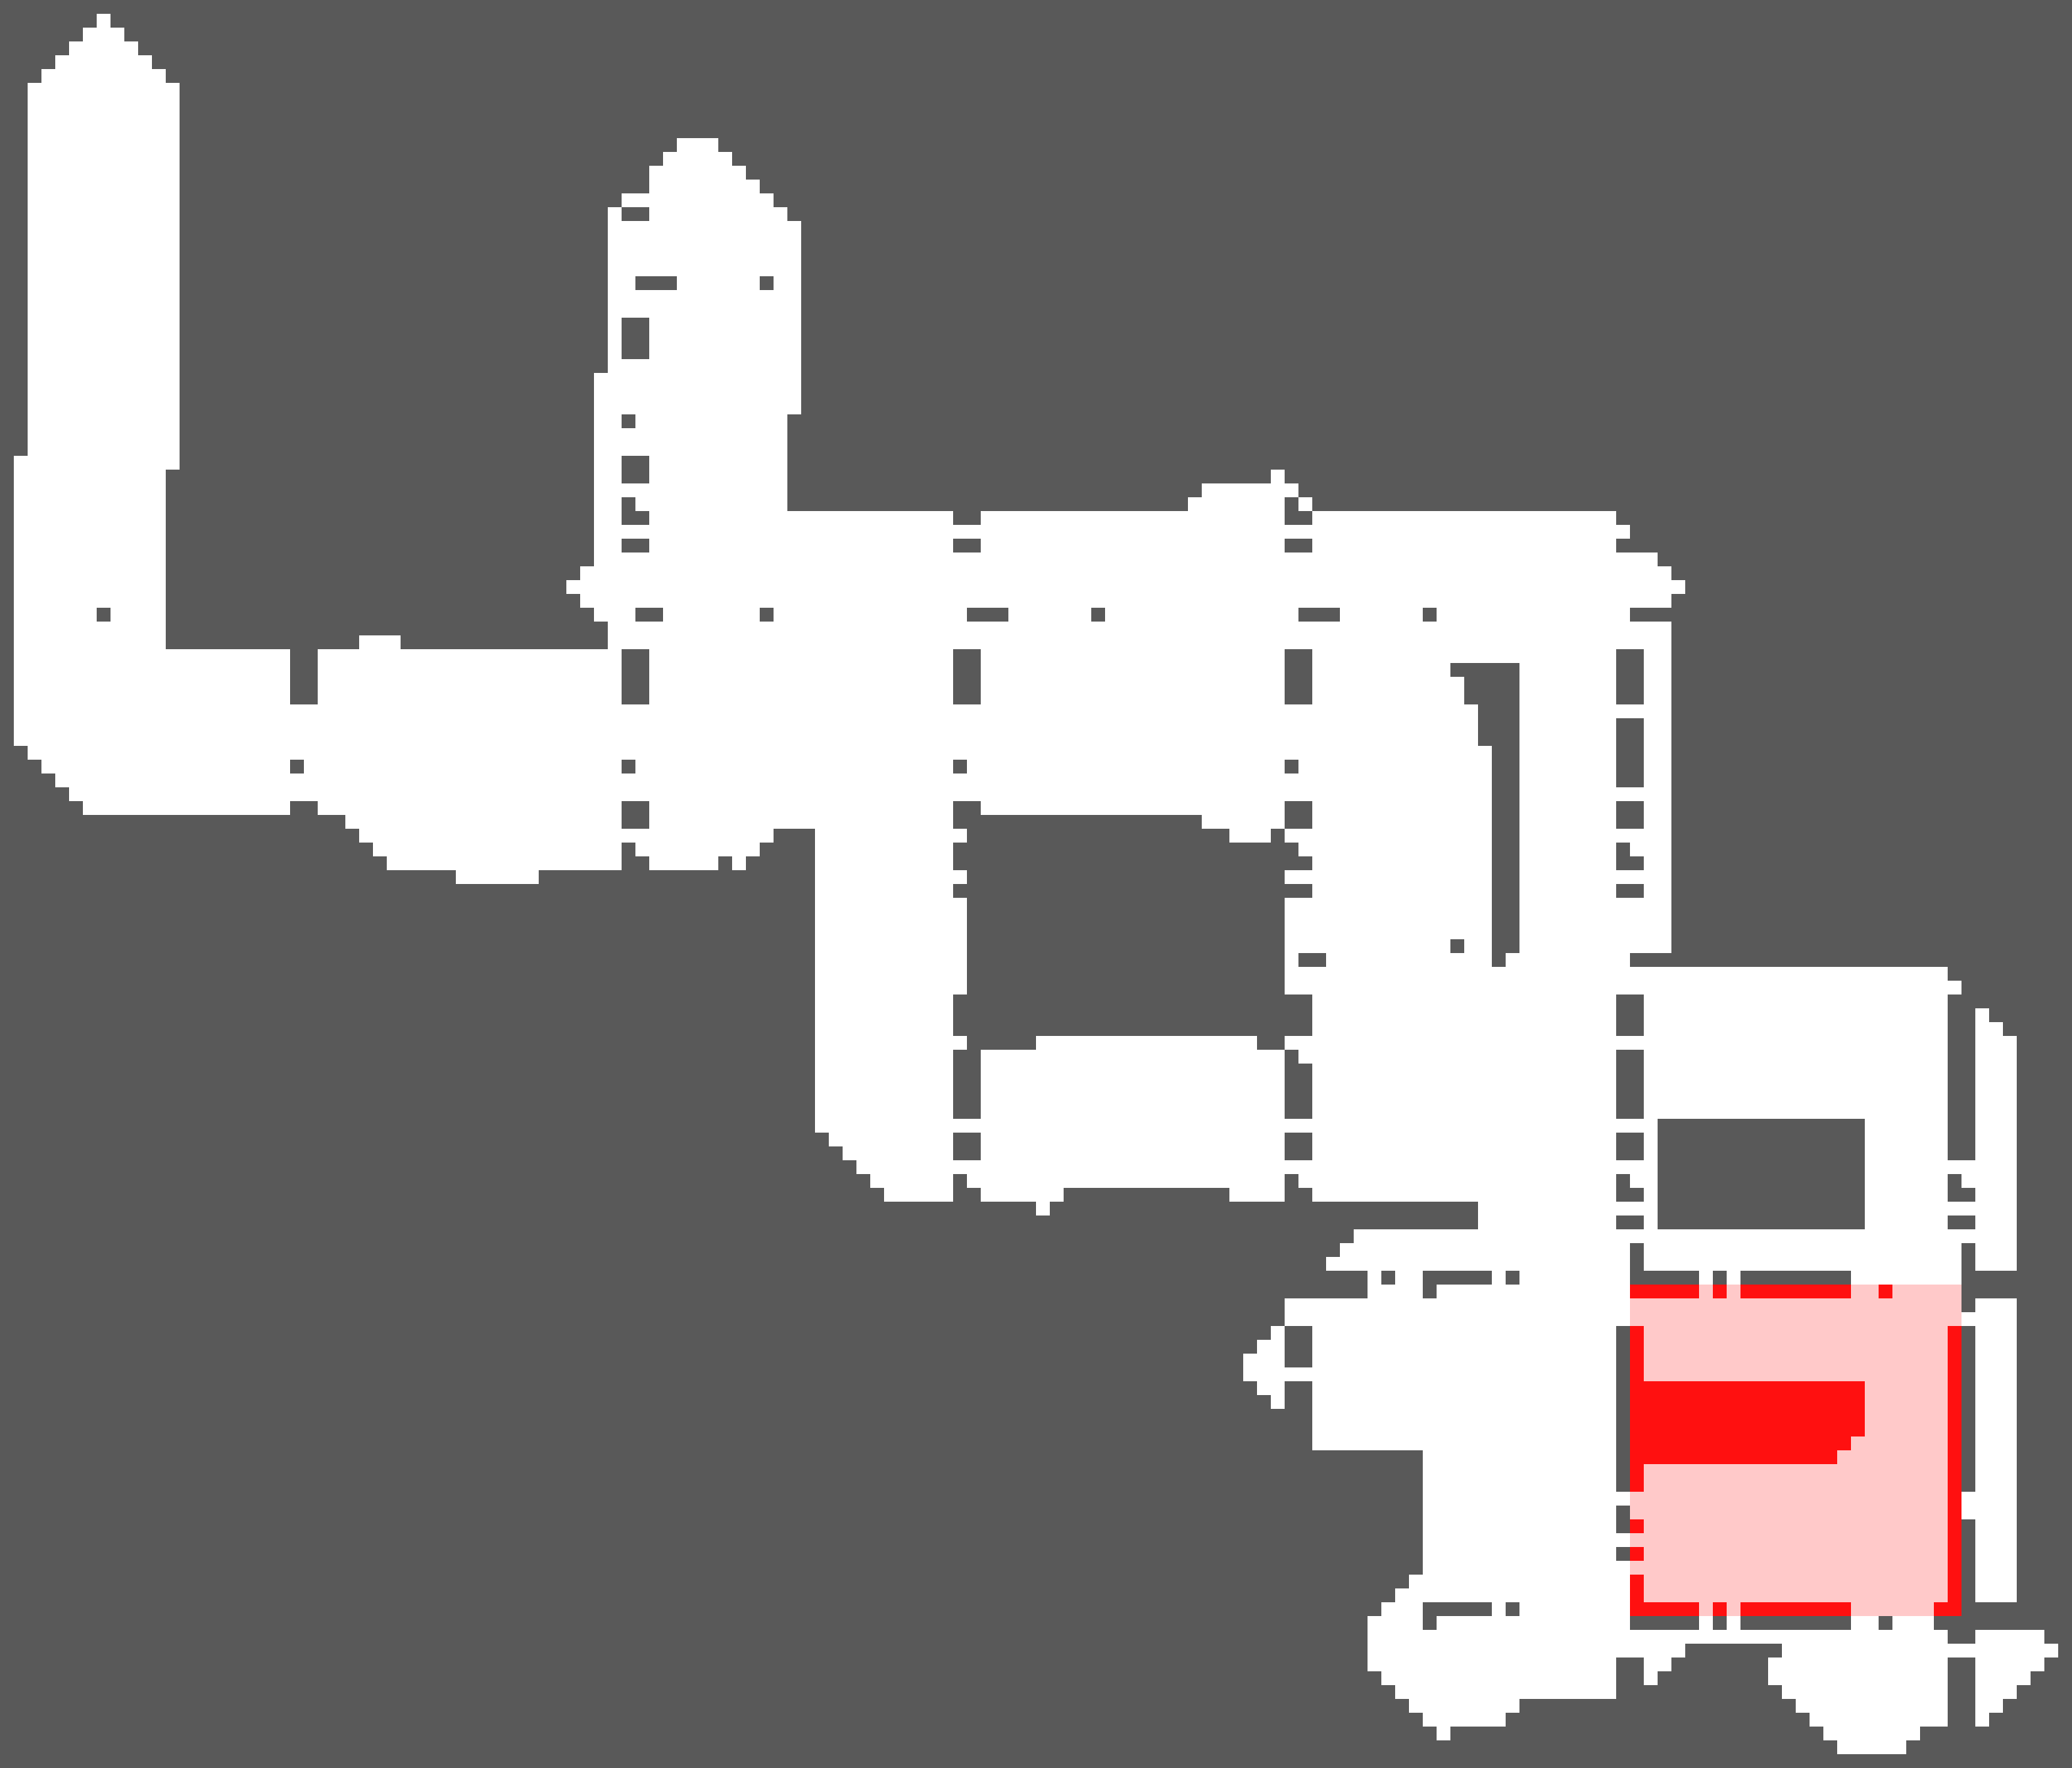
\includegraphics[width=125px]{bilder/karte3.png}
	\centering
	\caption{Beispiel für eine gestreckte Karte basierend auf einer 24x24 Welt }
	\label{fig:kartenwiederholung}
\end{figure}
